\documentclass{article}

\usepackage{jragonfyre}
\theoremstyle{remark}
\newtheorem*{question}{Question}
\newtheorem*{fact}{Fact}
\newtheorem{exercise}{Exercise}

\newcommand\diam{\operatorname{diam}}

\title{Bergelson Notes 7/2}
\author{Jason Schuchardt}

\begin{document}

\maketitle

We know by now that $\RR^n$ is complete with respect
to any of these metrics:
\[\rho_p(x,y) = \sqrt[p]{\sum |x_i-y_i|^p}, \text{ $p\in [1,\infty]$.} \]

We also know that for $-\infty < a < b < \infty$,
\[ (C[a,b],\rho)\quad \rho(f,g) =\max_{x\in[a,b]} |f(x)-g(x)| \]
is a complete metric space.

Go on the internet and look at the Theorem of Sharkovsky.
There is a proverbial saying 

Which continuous mappings of $[0,1]$ do we want to call chaotic?
Note: It's not the function itself that is chaotic, it is 
the iteration of the function that is chaotic.

Contractions are not very chaotic, by the Banach fixed point 
theorem. One thing we might care about is 
\emph{sensitive dependence on initial conditions}.

\section{Features of ``chaos''}

What is the origin of the word ``chaos''?

Let $f:X\to X$, where $(X,d)$ is a compact metric space.
\begin{enumerate}
    \item Sensitive dependence on initial conditions.
        There exists $\epsilon > 0$, for all 
        $x,y\in X$, $x\ne y$, there exists $n\inN$
        \[
        d(f^n(x),f^n(y)) > \epsilon
        \]

        We know plenty of mappings that are not chaotic.
        For example contractions, isometries. 
    \item There exists $x\in X$ such that
        the semiorbit of $x$,
        \[ \set{f^n(x) : n\inN}, \]
        is dense.

        This condition prevents your function from being trivial
        on some part of your space.

    \item Periodic points of $f$ are dense in $(X,d)$.
\end{enumerate}

This is a decent definition of chaotic.

Remind me on Thursday to define distal.

What are examples of chaotic functions?

Logistic mapping, $f(x) = ax(1-x)$, but for which parameters?
$a = 4$ is a good choice of parameter. See Figure 
\ref{fig:logistic}.
\begin{figure}
    \centering
    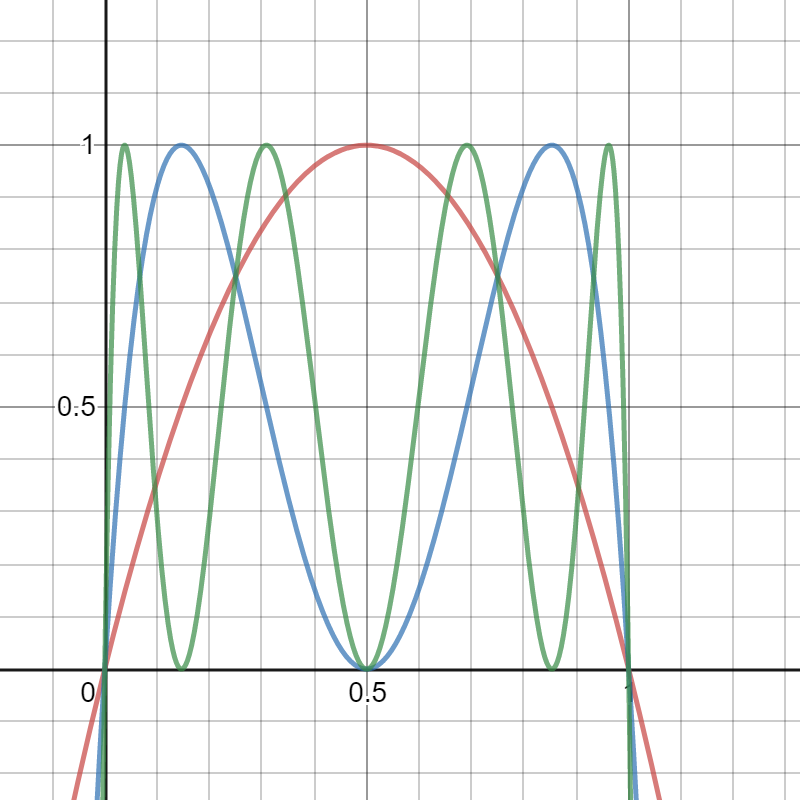
\includegraphics[width=0.6\textwidth]{desmos-graph-logistic.png}
    \caption{Three iterates of the logistic function}
    \label{fig:logistic}
\end{figure}

Also the tent map, $f(x) = -2|x-1/2| + 1$.

What is the first iteration of the tent map? It is two tents
with peaks at $1/4$, $3/4$.
$f^3$ will have $4$ peaks. See Figure 
\ref{fig:tent}.
\begin{figure}
    \centering
    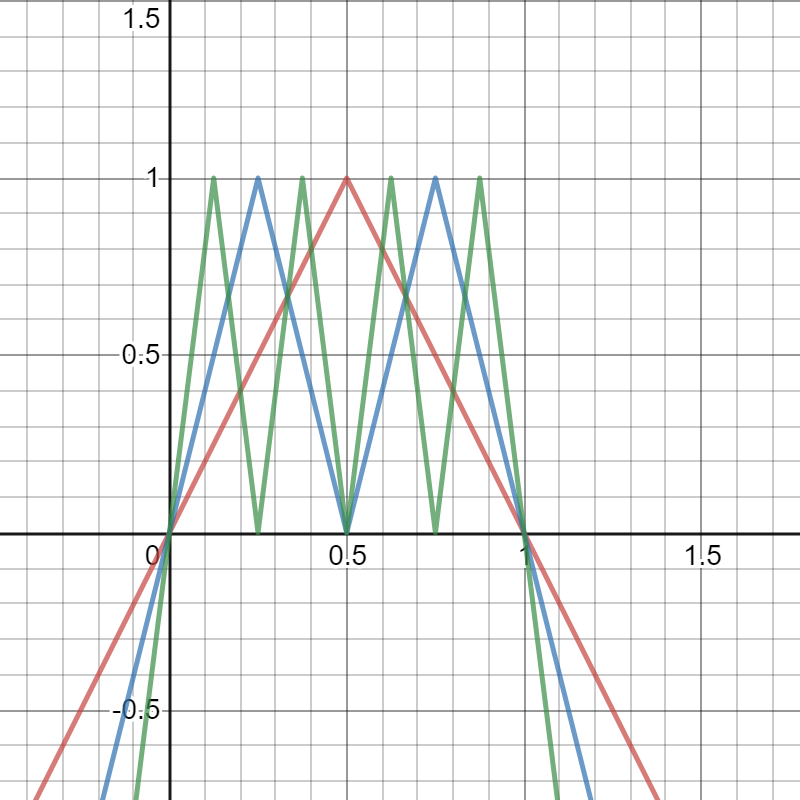
\includegraphics[width=0.6\textwidth]{desmos-graph.png}
    \caption{Three iterates of the tent map}
    \label{fig:tent}
\end{figure}

\begin{exercise}
    Verify the three conditions for these two maps.
\end{exercise}

How do we know that there are transitive points? (I.e.,
those points satisfying property (3), having dense orbit).

We can also consider the map $x\mapsto 2x$ on $S^1$. It 
might be easier to show these properties for this map.
This map is somehow isomorphic to the tent map.
We will write this map as $f(x) = 2x\mod{1}$

\begin{exercise}
    Which sets in $\RR$ can be sets of discontinuity of 
    monotone functions? We know that they must be countable,
    but which countable sets can occur? Can they be dense?
\end{exercise}

\section{How can we define an isomorphism}

What is an isomorphism of metric spaces? 
What is an isomorphism in general mathematics?

It depends on your objects. 
It is a map that preserves the properties of the objects.

Is $(0,1)$ isomorphic to $\RR$ as metric spaces? 
You should be a bit uncomfortable, since $(0,1)$ is bounded,
but $\RR$ is unbounded. Are they isomorphic though?

We can project the circle onto the line by projecting from
one of the poles.

This gives a topological isomorphism, which we call a 
\emph{homeomorphism}. This map gives a continuous renaming of the 
points, and the inverse is also continuous.
You can also take the lower half of a circle and project
from the center.

This example can be generalized to a mapping
projecting $S^n\setminus {\text{ north pole}}$ onto
the tangent plane to its south pole. This map is called
the stereographic projection. It establishes the homeomorphism
of the punctured $n$-sphere with $\RR^n$.

Do you know what a conformal mapping is? It is an angle 
preserving map. What is angle? What is an angle on the
sphere?

Suppose you take two intersecting curves on the sphere,
how do we measure the angle between them? Take the tangent
vector and then take the dot product of these vectors to
compute the angle.

\begin{exercise}
    Prove that stereographic projection is a conformal mapping.

    Where is the conformality in the $1$-dimensional picture?
\end{exercise}

Question: Is stereographic projection conformal in $n$-dimensional
space?

\begin{exercise}
    Find a good formula for stereographic projection, and
    then generalize it to $\RR^n$.
\end{exercise}

\section{$2x\mod{1}$}

Why is the transformation of the circle, 
$Tx:=2x \mod{1}$ so obviously chaotic? (See Figure
\ref{fig:2x-mod-1}.)
\begin{figure}
    \centering
    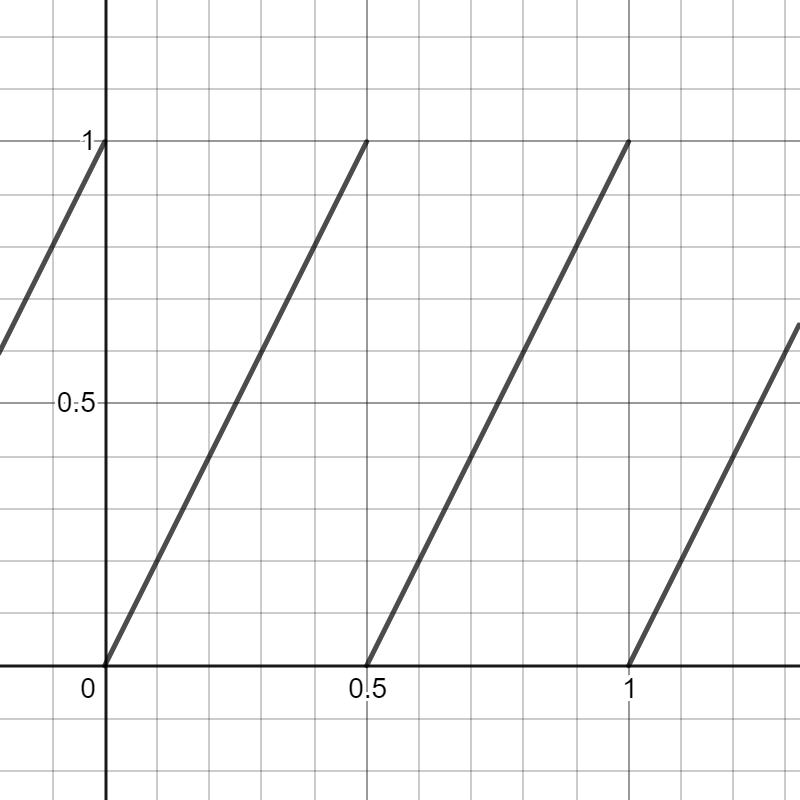
\includegraphics[width=0.6\textwidth]{desmos-graph-2x-mod-1.png}
    \caption{$2x\mod{1}$}
    \label{fig:2x-mod-1}
\end{figure}


Consider the binary expansion:
\[\label{eqn:binrep}\tag{*}
    x=\sum_{i=1}^\infty \frac{b_i}{2^i} \to (b_1(x),b_2(x),\ldots)\]
$b_i\in\set{0,1}$.

\begin{exercise}
    Which points have nonunique expansion \eqref{eqn:binrep}? 
    Can we have three different expansions? Five different
    expansions?

    Check that one of the expansion will be finite if 
    there are multiple expansions.
\end{exercise}

The map $2x\mod{1}$ when we encode $x$ as a binary expansion
corresponds to shifting the binary sequence:
\[ (b_1,b_2,\ldots) \mapsto (b_2,b_3,\ldots).\]
This map on sequences is also obviously $2$ to $1$.

Let \[ X=\set{0,1}^\NN=\set{\text{all $0-1$ sequences}}.\]

\begin{remark}
Cantor sets are also important in fixed point theory, and if we 
behave we might talk about fractals.
\end{remark}

Let us discuss how to measure distance between elements in this
space? Let $x=(x_i)_{i\inN}$, $y\in(y_i)_{i\inN}$ be 
sequences in $X$. Then we can define a metric on $X$ by
\[ d(x,y) = \sum_{i=0}^\infty \frac{|x_i-y_i|}{2^i} \]
We want digits that are far away to weigh less.
Two sequences are close if their initial terms coincide.

The maximum distance between two sequences in this space is
$1$, which is achieved when two sequences are bitwise complements
of each other.

\begin{exercise}[Culture]
    What does it mean to say that there is
    ``writing on the wall.''
    It is from the Book of Daniel. The writing is Aramaic.
\end{exercise}

\begin{definition}
    If $X$ is a metric space, we define the \emph{diameter}
    of $X$
    \[\diam X = \sup_{x,y\in X} d(x,y). \]

    It would be wrong to say that the diameter is the maximum
    distance. It might not exist, like in $(0,1)$.
\end{definition}

The diameter of our space $X$ is $1$.

\begin{exercise}
    $(X,\rho)$ is a compact space.
\end{exercise}

Claim: $(X,\text{shift})$ is a chaotic system.
(If $f:X\to X$ is chaotic, then the pair $(X,f)$ is a chaotic
system). This definition of chaos is for the purposes of today.

\begin{exercise}
Look for periodic points, and points with dense orbit
for this system.

The points $(0,1,0,1,0,1,\ldots)$ and $(0,0,0,0,\ldots)$ were 
already mentioned.
\end{exercise}

Note that this metric is the analog of the $\rho_1$ metric,
$\rho_1(x,y) = \sum_{i=1}^n |x_i-y_i|$.

\begin{exercise}
    Take any other sequence and normalize the $|x_i-y_i|$ by 
    that sequence and see whether you have a homeomorphic 
    space.

    I.e., let $a=(a_n)_{n\inN}$ be any sequence in $\RR_{\ge 0}$
    such that $\sum_n a_n$ converges, then define
    \[ d_a(x,y) = \sum_n a_n|x_i-y_i|.\]
    Check that this is a metric, and see whether it is 
    homeomorphic or not.
\end{exercise}

\begin{exercise}
    Claim: $(X,\rho)$, where $X=2^\NN$, $2=\set{0,1}$,
    and $\rho(x,y) = \sum_{i} \frac{|x_i-y_i|}{2^i}$
    is homeomorphic to the classical Cantor set with
    the Euclidean distance.
\end{exercise}

Have you seen Smale's Horseshoe? It connects to chaos theory
and the Cantor set. Look it up.

\begin{question}
    Can we take a contraction, and change the definition
    by allowing the constant $c$ to not be less than $1$.
    Will they still not be chaotic?

    No: For example if $c=10^6$, we have already seen examples
    where it is not chaotic.
\end{question}

\begin{question}
    Is it sufficient to be locally expanding in order to be a
    chaotic map? For example, there is some $\delta > 0$, 
    $\epsilon > 0$ such that for $d(x,y) < \delta$, we have
    \[ d(f(x),f(y)) > (1+\epsilon) d(x,y)? \]

    Answer: Not sure.

    After some discussion, it seems like we might need to be
    a bit more careful about this. The tent function
    doesn't seem to be locally expanding, though it
    feels intuitively like it ought to be. 
    It's not obvious that periodic
    points exist either.
\end{question}


\begin{question}
    In the definition of chaos?
    Do we have to require that $f^n(x)\ne f(x)$ for any $n$?

    Answer: Discuss it next time. It is too early to discuss any
    of the examples from today.
\end{question}

Another chaotic mapping:
\[\bmat 2 & 1 \\ 1 & 1 \emat  : \TT^2\to \TT^2, \]
where $\TT^2=\TT\times \TT = S^1\times S^1=\RR^2/\ZZ^2$.
See Figure \ref{fig:torus}.
Similarly $\TT^n = \RR^n/\ZZ^n$. 

\begin{figure}
    \centering
    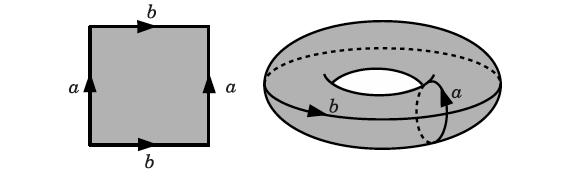
\includegraphics[width=0.8\textwidth]{torus.png}
    \caption{The 2-torus, $\TT^2$}
    \label{fig:torus}
\end{figure}

What is the metric on the torus? It is the distance on the
square (modulo identifications).

\[ \bmat 2 & 1 \\ 1 & 1 \emat \bmat x \\ y \emat 
= \bmat 2x + y \\ x + y \emat \in \TT^2 \]
This is one of many chaotic maps.

There is the baker's transformation, cut the square in half,
put the halves next to each other,
and squeeze into a square again. Also called the Arnold's cat 
transformation.

Any map of this kind is called a 
\emph{hyperbolic automorphism of the 
torus}. Why is it an automorphism? It's in the group 
theory sense. Why is it hyperbolic?

It has determinant one. Since the determinant is the product 
of the eigenvalues, one eigenvalue will be larger than $1$, 
and the other eigenvalue will be smaller than $1$ (in absolute
value). The eigenvalues may be complex.

What matters is that in one direction, things are expanding,
and in the other direction, things are contracting.

This is a good intuition for chaos: one direction expanding,
one contracting, and all in a bounded domain, so we get 
mixing.

\begin{exercise}
    Characterize those $2\times 2$ matrices that are hyperbolic.
\end{exercise}

Do you see the connection between this matrix
and Fibonacci numbers?

Let's start with
\[ \bmat 1 & 1 \\ 1 & 0 \emat^2 = \bmat 2 & 1 \\ 1 & 1 \emat \]
\[ \bmat 1 & 1 \\ 1 & 0 \emat^3 = \bmat 3 & 2 \\ 2 & 1 \emat \]
\[ \bmat 1 & 1 \\ 1 & 0 \emat^4 = \bmat 5 & 3 \\ 3 & 2 \emat \]
Q.E.D.

\begin{exercise}
    Establish formulas about the Fibonacci sequence using this
    matrix.

    Note that the eigenvalues are $\phi$, $-1/\phi$.
\end{exercise}

\section{Brouwer's fixed point theorem}

\begin{theorem}[Brouwer]
    Any continuous map $f:B_n\to B_n$
    has a fixed point, where $B_n$ is the closed unit ball
    in $\RR^n$. 
\end{theorem}

What proofs have you seen? For $C^1$ functions, or by algebraic
topology.

There's a good proof using combinatorics, via Sperner's lemma.
It is the best proof for us. 
You only need to be smart, not educated to understand it.
It is elementary in the sense of Richard Feynman:
\begin{quote}
    I am going to give what I will call an elementary
    demonstration. But elementary does not mean easy
    to understand. Elementary means that very little 
    is required to know ahead of time in order to understand
    it, except to have an infinite amount of intelligence.
    There may be a large number of steps that are hard 
    to follow, but to each does not require already knowing
    calculus or Fourier transforms.
\end{quote}

We could also formulate this theorem for the unit cube,
$[0,1]^n$. Why? Because they are homeomorphic.

What might be a more general domain we could formulate it for?

Maybe closed, bounded? (no two points) and connected?
(no the circle) 

Seminar: Convexity and its properties. Being comfortable with
convex sets in functional spaces.

\begin{definition}
    A \emph{convex body} in $\RR^n$ is a bounded, closed, convex set,
    with a nontrivial interior.

    A subset $S$ of $\RR^n$ is \emph{convex} if for all 
    $x,y\in S$ the line segment, $[x,y]\subset S$, 
    i.e. $(1-t)x+ty \in S$ for all $t\in [0,1]$.
\end{definition}


\begin{exercise}
    Theorem: Any convex body in $\RR^n$ is homeomorphic to 
    $B_n$.

    Picture: Take a point in the interior, every line through
    that point intersects the boundary in exactly two points.
\end{exercise}

\begin{exercise}
    Claim: Brouwer's theorem holds for any set in $\RR^n$
    which is homeomorphic to $B_n$.
\end{exercise}

\subsection{Sperner's Lemma}

Picture: A triangulation of a triangle.

\begin{definition}
    A \emph{triangulation} (of a triangle)
    is called simplicial, if any 
    two triangles either do not intersect, intersect in a
    common edge of both triangles (i.e., they share a side),
    or intersect at their vertices (a single common vertex only).

    Note that this implies that the triangles' interiors are all
    disjoint. Also note that triangulations have finitely
    many triangles.
\end{definition}

Call a $\set{1,2,3}$ labeling of vertices of a triangulation
(of a triangle)
\emph{special} if: 
\begin{enumerate}
    \item The vertices of the original triangle get 
        labeled $1$, $2$, and $3$ respectively. Call these vertices
        $A$, $B$, and $C$ respectively. 
    \item Any vertex on $AB$ gets either
        the label $1$ or $2$, and similarly for $BC$ and $AC$.
\end{enumerate}

\begin{theorem}[Sperner's lemma]
    For any special labeling of vertices in a simplicial
    triangulation, there exists a nontrivial subtriangle
    labeled $(1,2,3)$
\end{theorem}

The idea here is that we can start with a triangle, and 
then subdivide and label, and obtain a smaller triangle.
Iterating this process, we can get closer to a particular point.
(Perhaps a fixed point :)?) 

We have a map $f:[0,1]\to [0,1]$. 

We can subdivide $[0,1]$ into many subintervals, which we can 
label with $0$ and $1$. $0$ gets labeled $0$ and $1$ gets 
labeled $1$.

Every point of division gets labeled $0$ or $1$.
Then there are two adjacent points with left point labeled $0$
and right point labeled $1$.

This gives us a new proof of our fixed point lemma.
If any of the division points are fixed, we are done.
Otherwise, label the points $0$ if $f(x) > x$, and $1$ if 
$f(x)<x$. Then take a $0$-$1$ labeled interval, and subdivide
again. Be careful here! The endpoints of the interval might 
move past each other. You can fix this though.

Iterate the process, to get a sequence of descending intervals
whose diameter goes to $0$. The intersection is nonempty,
by compactness, and the point in the intersection will be a 
fixed point.

\begin{exercise}
    Fix this proof of the fixed point theorem via labelings.
\end{exercise}

\begin{exercise}
    Look up the game of Hex on the internet. Hex has a solution.

    Hex: We have a shape, covered by a tiling. One player 
    starts on one side, and tries to connect the sides.
    The other player tries to block.
\end{exercise}

Why are we talking about Hex? Because Brouwer's theorem is 
equivalent to the theorem that Hex has a winner.

Consider the map
\[ x\mapsto Ax + b, \quad x,b\in\RR^n.\]
We are interested in finding fixed points here.
What conditions on $A$ guarantee a fixed point? 

It depends on the metric we choose. In some metrics, it is 
a contraction, in some metrics, it is not.

\begin{exercise}
    What are the conditions for $Ax+b$ to be a contraction,
    if you endow $\RR^n$ with the metric $\rho_2$? $\rho_1$?
    $\rho_\infty$?
\end{exercise}




\end{document}